\chapter[Lecture 17]{}\label{lec17}

\section*{Elastic Wave in Cubic Crystals}
\begin{figure}[H]
\centering
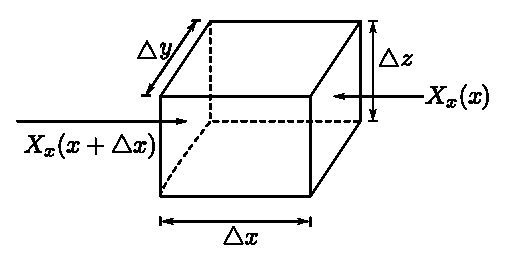
\includegraphics{images/lecture17/fig1.eps}
\end{figure}
On an infinitesimally small volume $\Delta x \cdot \Delta y \cdot \Delta z$, the $\phi$ Stress on the face $x$ is $-X_{x}(x)$ and at $(x+\Delta x)$, it is $X_{x}(x+\Delta x)$. The Net force can be expressed as $[X_{x}(x+\Delta x)-X_{x}(x)]^{\Delta y\Delta z}=\dfrac{\partial X_{x}}{\partial x} \cdot \Delta x \cdot \Delta y \cdot \Delta z$
$$
\therefore \text{ Force } =\dfrac{\partial X_{x}}{\partial x}\Delta x \cdot \Delta y \cdot \Delta z
$$
Similarly $x$-component of force due to stress on other surfaces are,
$$
\frac{\partial X_{y}}{\partial y}\cdot \Delta y\cdot \Delta x\cdot \Delta z\quad \text{and}\quad \frac{\partial X_{z}}{\partial z}\cdot \Delta z\cdot \Delta x\cdot \Delta y
$$
$\therefore$ The total force
$$
F_{x}=\left(\frac{\partial X_{x}}{\partial x}+\frac{\partial X_{y}}{\partial y}+\frac{\partial X_{z}}{\partial z}\right)\Delta x \Delta y \Delta z
$$
if the acceleration is $\dfrac{\partial^{2}u}{\partial z^{2}}$ and density is $\rho$.

Mass = $\rho dV$, $dV=\Delta x \Delta y \Delta z$
\begin{gather*}
\therefore\quad \fbox{$\rho \dfrac{\partial^{2}u}{\partial t^{2}}=\dfrac{\partial X_{x}}{\partial x}+\dfrac{\partial X_{y}}{\partial y}+\dfrac{\partial X_{z}}{\partial_{z}}$}\\
\text{[In a Cube]}\Rightarrow = C_{11}\dfrac{\partial e_{xx}}{\partial x}+C_{12}\left(\dfrac{\partial e_{yy}}{\partial x}+\dfrac{\partial e_{zz}}{\partial x}\right)+C_{44}\left(\dfrac{\partial e_{xy}}{\partial y}+\dfrac{\partial e_{xz}}{\partial z}\right)\\
\fbox{$\rho \dfrac{\partial^{2}}{\partial l^{2}}=C_{11}\dfrac{\partial^{2}u}{\partial x^{2}}+C_{44}\left(\dfrac{\partial^{2}u}{\partial y^{2}}+\dfrac{\partial^{2}u}{\partial z^{2}}\right)+(C_{12}+C_{44})\left(\frac{\partial^{2}v}{\partial x\partial y}+\dfrac{\partial^{2}w}{\partial x\partial z}\right)$}
\end{gather*}
$u$, $v$, $w$ are component of the displacement, $R$.

One can write down the corresponding equation for $\dfrac{\partial^{2}v}{\partial t^{2}}$ and $\dfrac{\partial^{2}w}{\partial t^{2}}$.
$$
\fbox{$\rho \dfrac{\partial^{2}w}{\partial z^{2}}=C_{11}\dfrac{\partial^{2}w}{\partial z^{2}}+C_{44}\left(\dfrac{\partial^{2}w}{\partial x^{2}}+\dfrac{\partial^{2}w}{\partial y^{2}}\right)+(C_{12}+C_{44})\left(\dfrac{\partial^{2}u}{\partial x\partial z}+\dfrac{\partial^{2}v}{\partial y\partial z}\right)$}
$$

\section*{Wave in [100] Direction}

For a wave moving in [100] direction, the wave equation will be $u=u_{0}\exp [i(k_{x}-wt)]$ $k=\dfrac{2\pi}{\lambda}$ for longitudinal wave.

Substituting this in the wave equation we get
$$
w^{2}\rho=C_{11}k^{2}
$$
$\therefore$ longitudinal wave velocity, $v_{s}=\dfrac{w}{k}$

$w=2\pi \nu$, $v_{S}=v_{\lambda}$, $k=\dfrac{2\pi}{\lambda}$
$$
\therefore\quad \fbox{$v_{S}=\sqrt{\dfrac{C_{11}}{\rho}}$}
$$
\begin{align*}
e_{xx} &= \dfrac{\partial u}{\partial x}\quad e_{yy}=\dfrac{\partial v}{\partial y}\quad e_{zz}=\dfrac{\partial w}{\partial z}\\
e_{xy} &= \dfrac{\partial u}{\partial y}+\dfrac{\partial v}{\partial x}\tag{*}
\end{align*}
{\bf For a transverse or Shear wave}
$$
v=v_{0}\exp [i(kx-wt)]
$$
For this we need to use equation for $\dfrac{\partial^{2}v}{\partial t^{2}}$ which is
$$
\fbox{$\rho\dfrac{\partial^{2}v}{\partial t^{2}}=C_{11}\dfrac{\partial^{2}v}{\partial y^{2}}+C_{44}\left(\dfrac{\partial^{2}v}{\partial x^{2}}+\dfrac{\partial^{2}v}{\partial z^{2}}\right)+(C_{12}+C_{44})\left(\dfrac{\partial^{2}u}{\partial x\partial y}+\dfrac{\partial^{2}w}{\partial y\partial z}\right)$}
$$
This gives 
$$
w^{2}_{\rho}=C_{44}k^{2}\quad a, \ \fbox{$v_{S}=\sqrt{\dfrac{C_{44}}{\rho}}$}
$$
{\bf For an wave in [110] direction.}

Shear wave propagates in the $xy$-plane with particle displacement in $z$-direction.
\begin{align*}
& w=w_{0}\exp[i(k_{x}x++++k_{y}y-wt)]\\
\Rightarrow & \fbox{$w^{2}\rho=C_{44}(k^{2+}_{x}+k^{2}_{y})=C_{44}k^{2}$}
\end{align*}
For the wave in my plane
\begin{align*}
u &= u_{0}\exp [i(k_{x}x+k_{y}y-wt)]\\
\text{and}\quad v &= v_{0}\exp [i(k_{n}x+k_{y}y-wt)]
\end{align*}
We get
$$
\fbox{
$
\begin{array}{l}
w^{2}\rho u = (C_{11}k_{x^{2}}+C_{44}k_{y^{2}})u+(C_{12}+C_{44})k_{a}k_{y}v\\
w^{2}\rho v = (C_{11}k^{2}_{y^{2}}+C_{44}k_{x^{2}})v+(C_{12}+C_{44})k_{x}k_{y}u
  \end{array}$}
$$
\fbox{$k_{x}=k_{y}=\dfrac{k}{\sqrt{2}}$}.

\smallskip

To get a solution of above two equations.
$$
\left|
\begin{array}{lr}
C-w^{2}\rho+\frac{1}{2}(C_{11}+C_{44})k^{2} & \frac{1}{2}(C_{12}+C_{44})k^{2}\\[5pt]
\frac{1}{2}(C_{12}+C_{44})k^{2} & -w^{2}\rho+\frac{1}{2}(C_{11}+C_{44})k^{2}
\end{array}
\right|=0
$$
The roots of the equations are -
$$
\fbox{$w^{2}\rho =\frac{1}{2}(C_{11}+C_{12}+2C_{44})k^{2}$} \ ;\quad \fbox{$w^{2}\rho=\frac{1}{2}(C_{11}-C_{44})k^{2}$}
$$
Substitute 1st root in the above equation $\to$
\begin{align*}
\frac{1}{2}(C_{11}+C_{12}+2C_{44})k^{2}u &= \frac{1}{2}(C_{11}+C_{44})k^{2}u+\frac{1}{2}(C_{12}+C_{44})k^{2}v\\
\Rightarrow u &= v
\end{align*}

Thus, the particle displacement is along [110] direction which is the wave propagations direction

$\to$ longitudinal wave.

$ma=F-mg$
\begin{figure}[H]
\centering
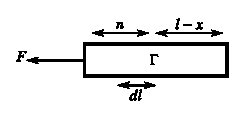
\includegraphics[scale=1.5]{images/lecture17/fig2a.eps}
\end{figure}
\begin{align*}
\text{net force } &= \frac{x}{l}(F-\cancel{mg})=F-T(a)-\cancel{\dfrac{mx}{l}g}\\
T(X) &= F\left(\frac{l-x}{l}\right)
\end{align*}
\begin{align*}
\dfrac{\frac{T}{A}}{\frac{dx}{dx}}-Y &= \dfrac{F}{AYl}(l-x)dx=d\Delta x\\[2pt]
\Delta x &= \int\limits^{l}_{x=0}\\[2pt]
&= \frac{F}{Ay\cancel{l}}\cdot \dfrac{\cancel{l^{2}}}{2}\\[2pt]
\text{Strain } &= \dfrac{F}{2AY}\\[2pt]
\text{Extension } &= \dfrac{Fl}{2AY}
\end{align*}

\eject

For second solution -
\begin{align*}
& \frac{1}{2}(C_{11}-C_{12})k^{2}u=\frac{1}{2}(C_{11}+C_{44})k^{2}u+\frac{1}{2}(C_{12}+C_{44})k^{2}v\\[2pt]
& \frac{1}{2}(C_{12}+C_{44})k^{2}v=\frac{1}{2}(C_{11}-C_{12}-C_{11}-C_{44})k^{2}u=-\frac{1}{2}(C_{12}+C_{44})k^{2}u\\[2pt]
&\Rightarrow \fbox{$u=-v$} \text{ Desplacement direction $[1\overline{1}0]$}\\[2pt]
&\Rightarrow \text{ transverse wave.}
\end{align*}
{\bf In General :} There are three normal modes of wave motion Two transverse and one longitudinal.

For a wave propagating in directions other than high symmetry axis $[100] \ [110] \ [111]$, the displacement may not be exactly parallel or perpendicular to $\overrightarrow{k}$.

\medskip
\noindent
{\bf Temperature :} Increase temperature, stiffness constant decreases.

Stiffness depends on the strength of bonding.

\section*{Crystal Vibration}

(1) When a wave propagates in some direction in a solid - Say [100], [110], [111] etc., the atoms in the entire plane perpendicular to propagation direction move {\em in-phase} with displacements parallel or perpendicular to the direction of wave motion.
\begin{itemize}
\itemsep=0pt
\item[$\to$] Problem is now one-dimensional.

\item[$\to$] Three modes; one longitudinal and two transverse.
\end{itemize}
$x=sa=$ the distance of the atom from some origin.

Assumptions :- Elastic response is linear function of force.
\begin{itemize}
\itemsep=0pt
\item[$\to$] Elastic energy is quadratic to displacement.

\item[$\to$] Linear terms in energy will vanish in equillibrium.

\item[$\to$] Higher order term (more than two) are too small to be considered.
\end{itemize}
If $u_{s}$ represents displacement of plan `$s$'

\eject

$\therefore$ Force plane `$s$' caused by displacement of plan $s\pm 1$ is proportional to the difference in displacement between the planes-
$$
\Rightarrow F_{s}=C(u_{s+1}-u_{s})+C(u_{s-1}-u_{s})
$$
following Hooke's law.

$C\to$ force constant between nearest neighbor planes.

Basically $u_{s}\sim e^{-i(w_{i}-kx)}\simeq l^{-i(wl-ksa)}$

Assume $F_{s}$ is acting on an atom on plane `$s$'.
$$
\therefore\quad \fbox{$M\dfrac{d^{2}u_{s}}{dt^{2}}=C(u_{s+1}+u_{s-1}-2us_{s})$}
$$
$M=$ mass of the atom.

Since the system is transmitting a wave, the solution of $u_{s}$ will have the form in time $-iwt$.

$\to$ Harmonic approximation
\begin{align*}
\therefore\quad & \dfrac{d^{2}u_{s}}{dt^{2}}=-w^{2}u_{s}\\
\therefore\quad & \fbox{$-Mw^{2}u_{s}=C(u_{s+1}+u_{s-1}+2u_{s})$}
\end{align*}
If the separation between the planes is `$a$', the space dependence can be written as \fbox{$u_{s\pm 1}=ue^{ika(s\pm 1)}$}.

$k$ is the wave vector $=\dfrac{2\pi}{\lambda}$.

Substituting this, we get
$$
-w^{2}Mue^{iska}=Cu\left[e^{i(s+1)ka}+e^{i(s-1)ka}-2e^{iska}\right]
$$
Divide both sides by
\begin{gather*}
ui^{iska},\Rightarrow \fbox{$w^{2}M=-C[e^{ika}+e^{-ika}-2]$}\\
a, \fbox{$w^{2}=\dfrac{2C}{M}(1-\cos ka)$}\quad \text{or,}\quad \fbox{$w=\sqrt{\dfrac{4C}{M}}\left|\sin \dfrac{ka}{2}\right|$}
\end{gather*}
at $k=\pm \dfrac{\pi}{a}$, $\dfrac{dw}{dk}=\text{ Const. } \cos \dfrac{ka}{2}=0\Rightarrow \text{ Slop of $w$ is zero.}$
\begin{figure}[H]
\centering
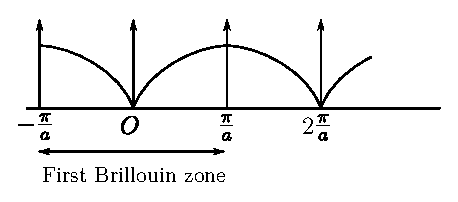
\includegraphics{images/lecture17/fig2.eps}
\end{figure}

Now $\dfrac{u_{s+1}}{u_{s}}=e^{ika}$\quad $a$ is the smallest separation between the planes.

$\therefore \ ka=\pm \pi$ would cover all independent values of the exponential.
$$
\therefore\quad -\pi <ka\leq \pi \Rightarrow \fbox{$-\dfrac{\pi}{a}<k\leq \dfrac{\pi}{a}$}
$$
This is defined as first Brillouin tone.
\begin{itemize}
\item If $k$ is outside this range; one can bring that inside the range by subtracting integral multiple of $\dfrac{2\pi}{a}$
\begin{gather*}
\text{e.g.}\quad k'=k-\dfrac{2\pi n}{a}\\
\dfrac{u_{s+1}}{u_{s}}=e^{ika}=e^{i2\pi n}\cdot e^{[i(ka-2\pi n)]}=e^{ik'a}
\end{gather*}
\fbox{$e^{i2\pi n}=1$}

\item At the boundary of the $BZ$, $k_{\max}=\pm \dfrac{\pi}{a}$, the solution,
$$
\fbox{$u_{s}=ue^{iska}\Rightarrow ue^{\pm is\pi}=u\cdot (-1)^{s}$}
$$
\begin{itemize}
\item[$\to$] $\therefore u$ represents a standing wave; NOT a travelling wave.

\item[$\to$] Alternate atom oscillate in opposite phase, as $u_{s}=\pm 1$ for even and odd `$s$'.
\end{itemize}
\end{itemize}
This situation is equivalent to Bragg condition for reflection of $x$-rays.

E.g. $k_{\max}=\pm \dfrac{\pi}{a}$\quad $a=d$\quad $k=\dfrac{2\pi}{\lambda}$
$$
\therefore\quad 2d\sin \theta=n\lambda \Rightarrow \text{For } \theta=\dfrac{\pi}{2}\text{ and } n=1\quad \fbox{$\lambda=2a$}
$$
$\therefore \ x$-rays cannot propagate in solid.

Through successive reflection back and forth at different lattice planes, it forms a standing wave.
\begin{itemize}
\item $n$ can be greater than $1$ for $x$-rays (electro-magnetic wave) whose propagation does not require an atom vibration.

\item Displacement amplitude for elastic wave is defined only through vibration of atoms.
\end{itemize}

\section*{Group Velocity}

Transmission velocity of a wave packet is called group velocity.
$$
\fbox{$v_{g}=\nabla_{k}w(k)$}
$$
This is the velocity of energy propagation.
$$
w=\sqrt{\dfrac{4C}{M}}\left|\sin \dfrac{ka}{z}\right|\Rightarrow \fbox{$V_{g}=\sqrt{\dfrac{Ca^{2}}{M}}\cos \dfrac{ka}{2}$}
$$
$v_{g}=0$ at $k=\pm \dfrac{\pi}{a} \ \Rightarrow \ $ Standing wave.

\medskip
\noindent
{\bf Long wavelength limit :} For $ka\ll 1$\quad $\cos ka\simeq 1-\dfrac{1}{2}(ka)^{2}$
$$
\therefore\quad \fbox{$w^{2}=\dfrac{C}{M}k^{2}a^{2}$} \ \Rightarrow \ \fbox{$w\alpha k$}
$$
Frequency is directly proportional to wave vector.

$\therefore \ $ Velocity of sound is independent of frequency 

$v=\dfrac{w}{k}$ as in the case of elastic wave for $ka\ll 1$.

